\documentclass{beamer}
\usetheme{Frankfurt} % http://deic.uab.es/~iblanes/beamer_gallery/
\usecolortheme{dove}

\setbeamertemplate{navigation symbols}{}
\makeatletter
\setbeamertemplate{footline}
{%
  \pgfuseshading{beamer@barshade}%
  \ifbeamer@sb@subsection%
    \vskip-9.75ex%
  \else%
    \vskip-7ex%
  \fi%
  \begin{beamercolorbox}[ignorebg,ht=2.25ex,dp=3.75ex]{section in head/foot}
    \insertnavigation{\paperwidth}
  \end{beamercolorbox}%
  \ifbeamer@sb@subsection%
    \begin{beamercolorbox}[ignorebg,ht=2.125ex,dp=1.125ex,%
      leftskip=.3cm,rightskip=.3cm plus1fil]{subsection in head/foot}
      \usebeamerfont{subsection in head/foot}\insertsubsectionhead
    \end{beamercolorbox}%
  \fi%
}%
\setbeamertemplate{headline}{}
\makeatother

\usepackage[T1]{fontenc}
\usepackage[utf8]{inputenc}
\usepackage[ngerman]{babel}
\usepackage[autostyle = true, german = quotes]{csquotes} % Anführungszeichen

\usepackage{amsmath}
\usepackage{graphicx}
\usepackage{epstopdf}

\begin{document}

%\subject{Praktikum Multicore"=Programmierung}
\title{Projekt~6: Mehrgittermethoden}
\author{Florian Klemme \and Manuel Leßmann}
\date{17.~Februar 2016}

\frame{\titlepage}

\AtBeginSection[]{ % Do nothing for \section*
    \begin{frame}
        \frametitle{Agenda}
        \tableofcontents[currentsection]
    \end{frame}
}

%\section*{Agenda}
\begin{frame}
    \frametitle{Agenda}
    \tableofcontents
\end{frame}

\section{Jakobi- und Gauß-Seidel-Verfahren}
\subsection{Beschreibung}
\begin{frame}
    \frametitle{Jakobi und Gauß-Seidel}
    \begin{block}{Jakobi}
        \(u_{i,j}^{k} = (u_{i,j-1}^{k-1} + u_{i-1,j}^{k-1}
                       + u_{i,j+1}^{k-1} + u_{i+1,j}^{k-1}
                       + h^2 \cdot f(i \cdot h, j \cdot h)) \mathbin{/} 4\)
    \end{block}
    \begin{block}{Gauß-Seidel}
        \(u_{i,j}^{k} = (u_{i,j-1}^{k} + u_{i-1,j}^{k}
                       + u_{i,j+1}^{k-1} + u_{i+1,j}^{k-1}
                       + h^2 \cdot f(i \cdot h, j \cdot h)) \mathbin{/} 4\)
    \end{block}
    \begin{center}
        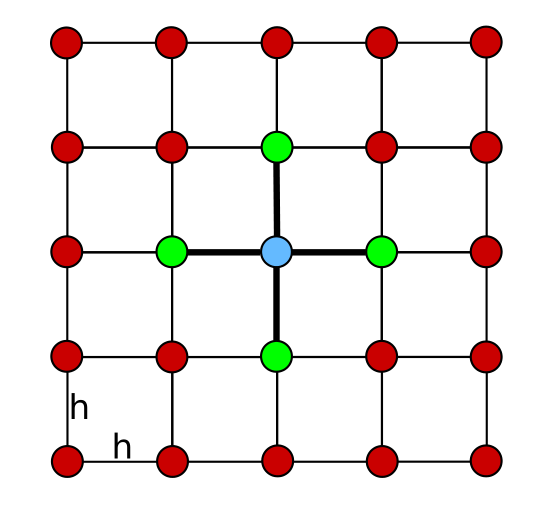
\includegraphics[width=0.4\textwidth]{jakobi-grid}
    \end{center}
\end{frame}

\begin{frame}
    \frametitle{Jakobi und Gauß-Seidel}
    \begin{block}{Abbruchbedingungen}
        \begin{itemize}
            \item Maximale Anzahl an Iterationen
            \item Maximale Änderung zwischen zwei Iterationen unterschreitet Grenzwert
        \end{itemize}
    \end{block}
    \begin{block}{Qualitätsmetriken}
        \begin{itemize}
            \item Maximaler Fehler zur analytischen Lösung
            \item Mittlerer Fehler zur analytischen Lösung
            \item Laufzeit des Algorithmus
        \end{itemize}
    \end{block}
\end{frame}

\subsection{Parallelisierung mit OpenMP}
\begin{frame}
    \frametitle{Parallelisierung Jakobi}
    Trivial parallelisierbar:
    \begin{itemize}
        \item Keine Datenabhängigkeiten innerhalb einer Iteration
        \item Reduktion der Abbruchbedingung
        \item Statische Lastverteilung, da jedes Arbeitspaket gleich groß ist
        \item Ping-Pong-Verfahren zum effizienten Zugriff auf die vorherige Iteration
    \end{itemize}
    Aber:
    \begin{itemize}
        \item Hoher Overhead, da eine einzelne Iteration v.a. bei groben Gittern nicht sehr lange dauert
    \end{itemize}
\end{frame}

\begin{frame}
    \frametitle{Parallelisierung Jakobi: Effizienz}
    \framesubtitle{1000 Iterationen}
    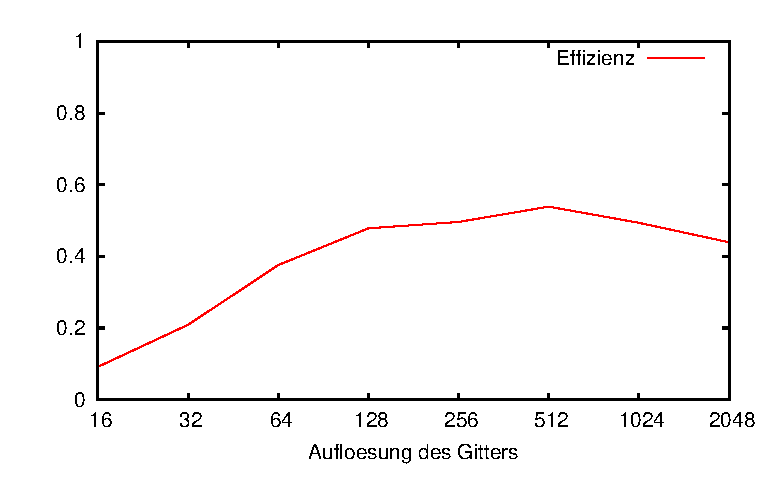
\includegraphics[width=\textwidth]{plots/effizienzjakobi}
\end{frame}

\begin{frame}
    \frametitle{Parallelisierung Gauß-Seidel}
    Datenabhängigkeiten innerhalb einer Iteration!
    \begin{itemize}
        \item[$\rightarrow$] Neuer Wert ist abhängig von den Nachbarn links und oberhalb aus der aktuellen Iteration.
    \end{itemize}
    Also: keine triviale Methode möglich.
\end{frame}

\begin{frame}
    \frametitle{Ansatz: Wavefront-Muster}
    \begin{center}
        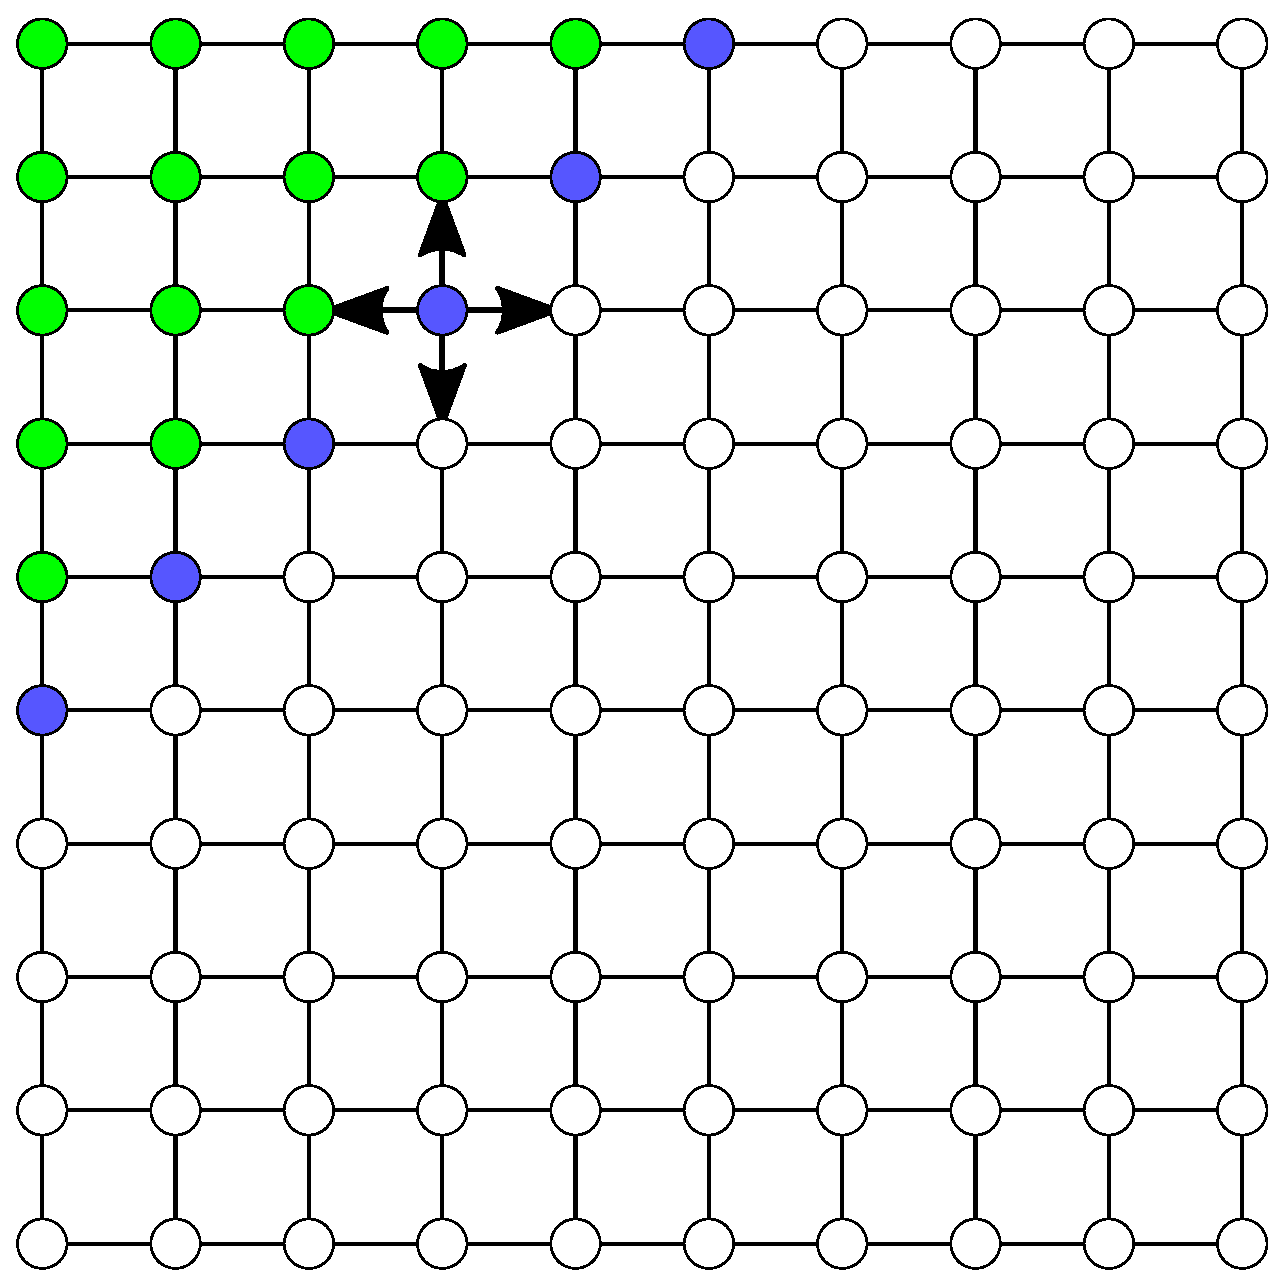
\includegraphics[width=0.5\textwidth]{wavefront-datadependencies}
    \end{center}
\end{frame}

\begin{frame}
    \frametitle{Ansatz: Wavefront-Muster}
    \begin{columns}
        \begin{column}{0.5\textwidth}
            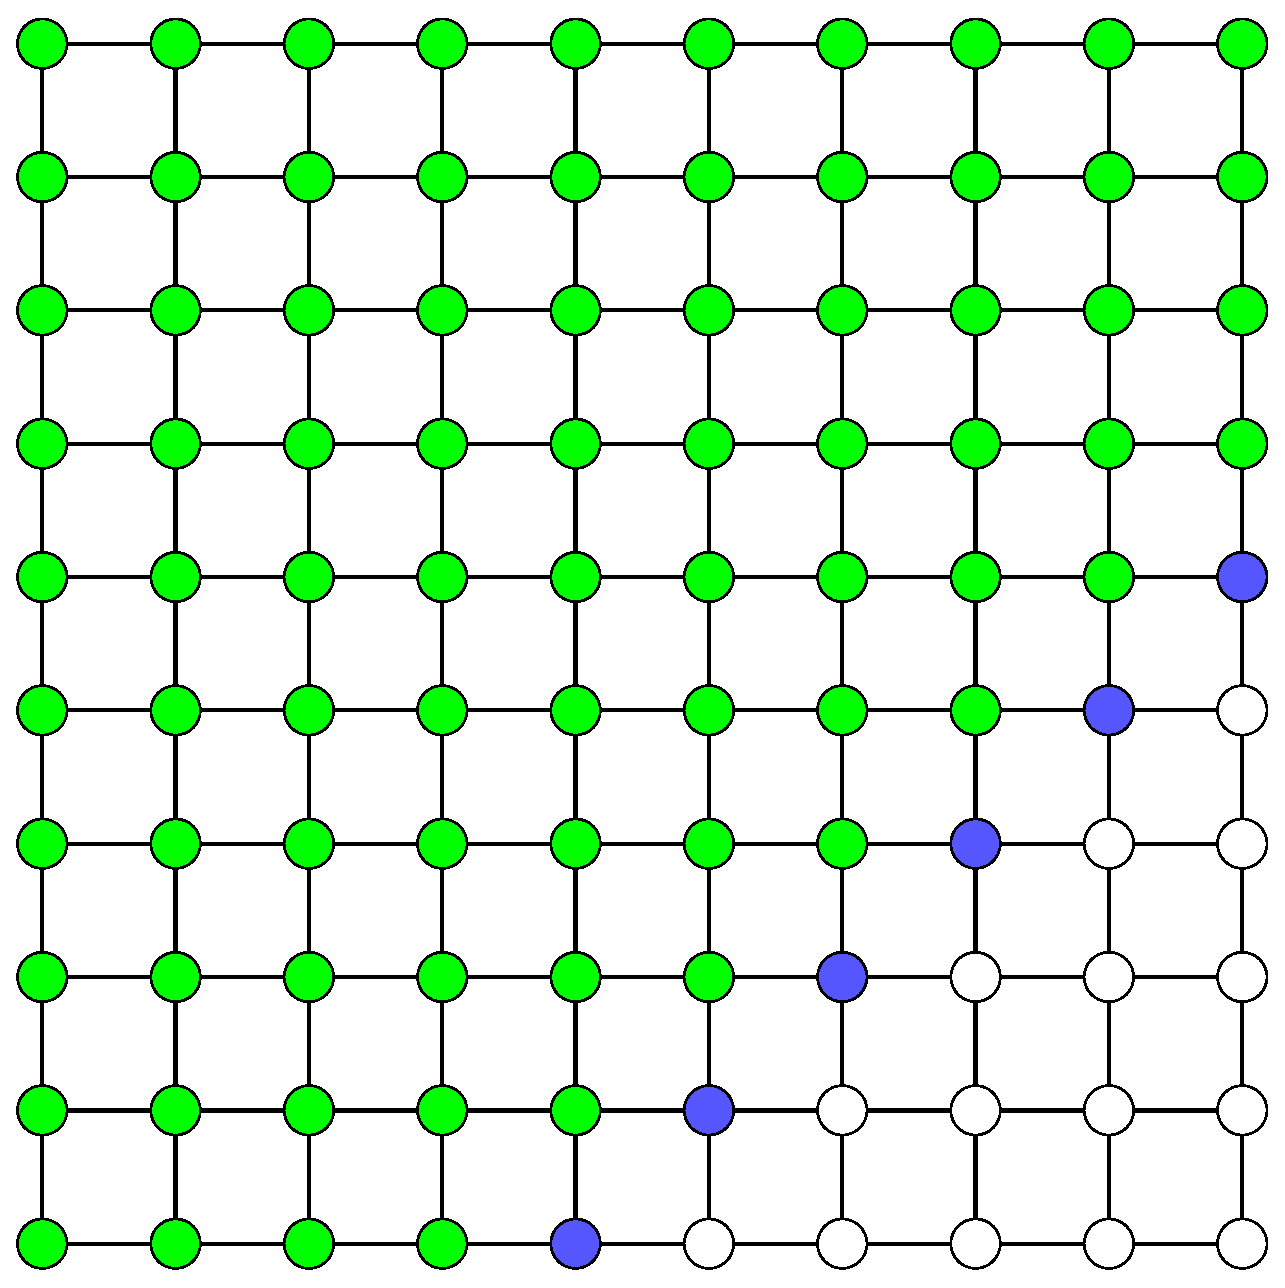
\includegraphics[width=\textwidth]{wavefront1}
            \begin{center}
                Iteration $n$
            \end{center}
        \end{column}
        \begin{column}{0.5\textwidth}
            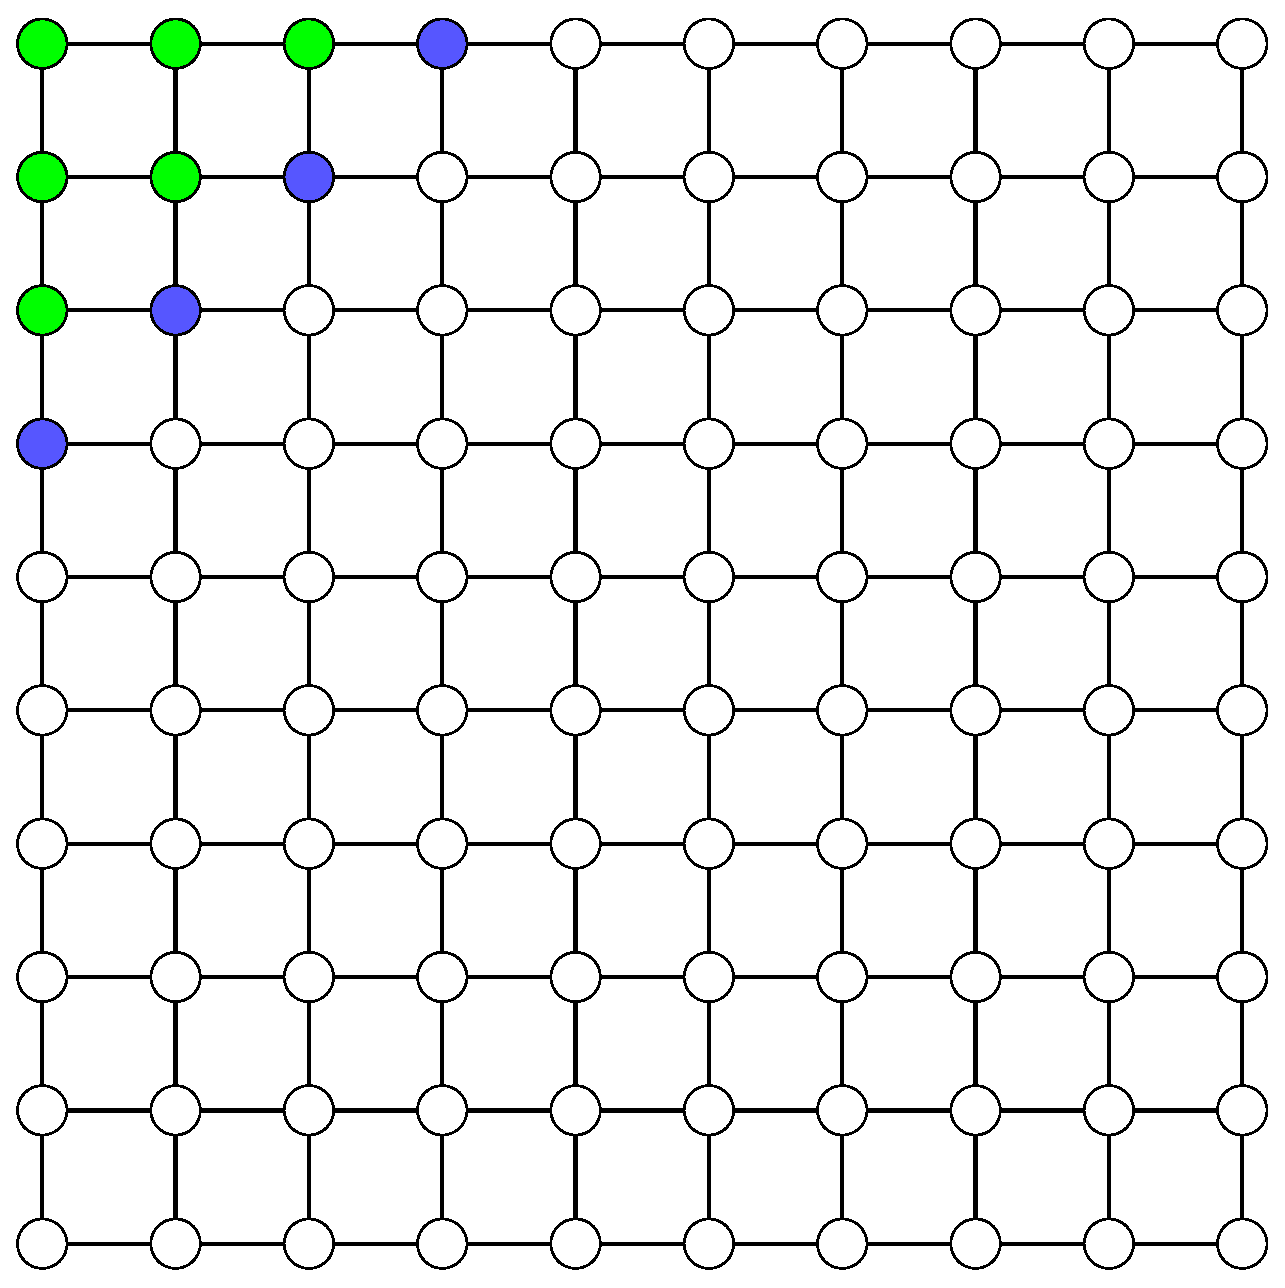
\includegraphics[width=\textwidth]{wavefront2}
            \begin{center}
                Iteration $n+1$
            \end{center}
        \end{column}
    \end{columns}
\end{frame}

\begin{frame}
    \frametitle{Ansatz: Wavefront-Muster}
    Probleme:
    \begin{itemize}
        \item Die Granularität der Arbeitspakete ist zu fein
        \item Schlechte Cache-Effizienz innerhalb eines Threads
    \end{itemize}
    Lösung:
    \begin{itemize}
        \item Zusammenfassen von Arbeitspaketen
    \end{itemize}
\end{frame}

\begin{frame}
    \frametitle{Wavefront-Gruppierung}
    \begin{columns}
        \begin{column}{0.5\textwidth}
            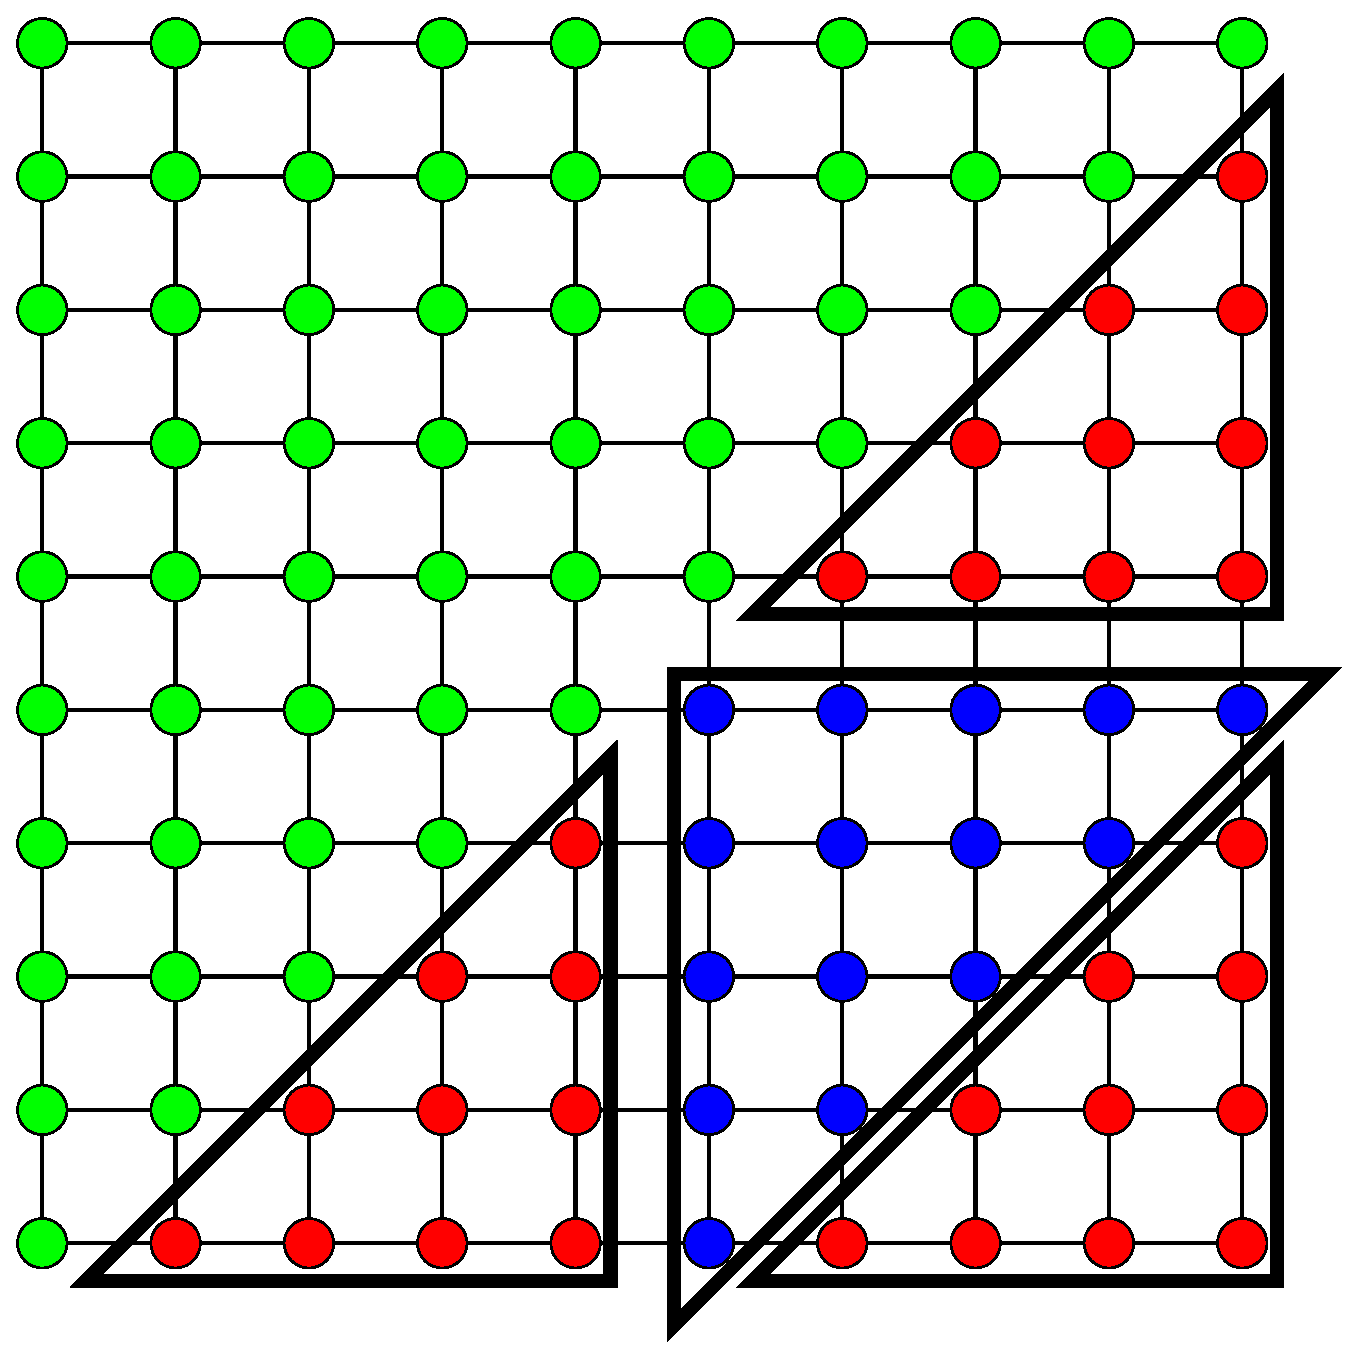
\includegraphics[width=\textwidth]{triangles1}
            \begin{center}
                Iteration $n$
            \end{center}
        \end{column}
        \begin{column}{0.5\textwidth}
            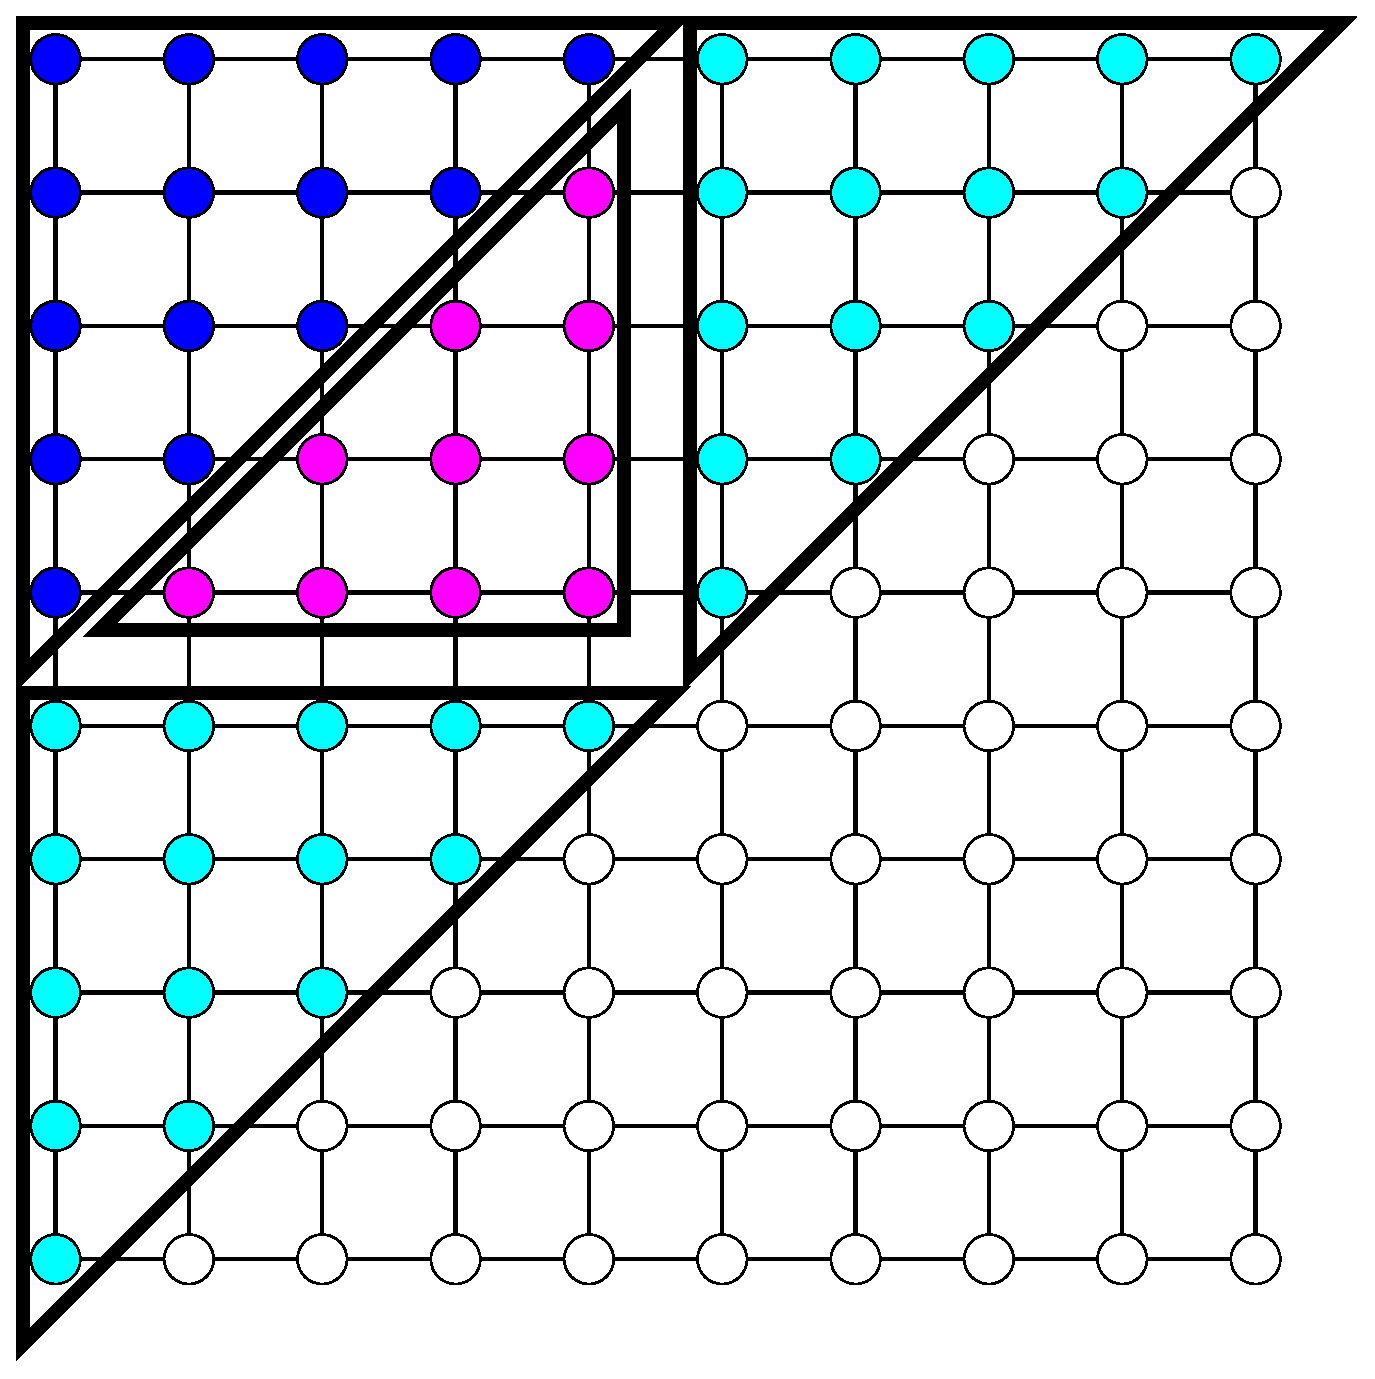
\includegraphics[width=\textwidth]{triangles2}
            \begin{center}
                Iteration $n+1$
            \end{center}
        \end{column}
    \end{columns}
\end{frame}

\begin{frame}
    \frametitle{Parallelisierung Gauß-Seidel: Effizienz}
    \framesubtitle{1000 Iterationen}
    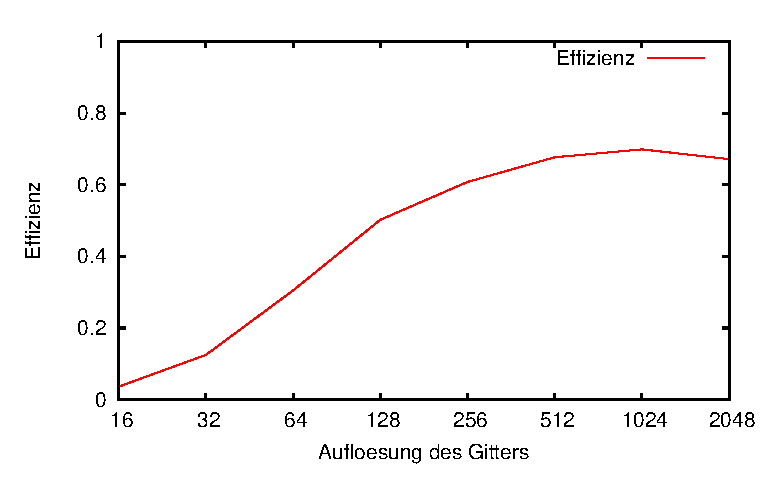
\includegraphics[width=\textwidth]{plots/effizienzgaussseidel}
\end{frame}

\subsection{Konvergenz}
\begin{frame}
    \frametitle{Konvergenz der Verfahren}
    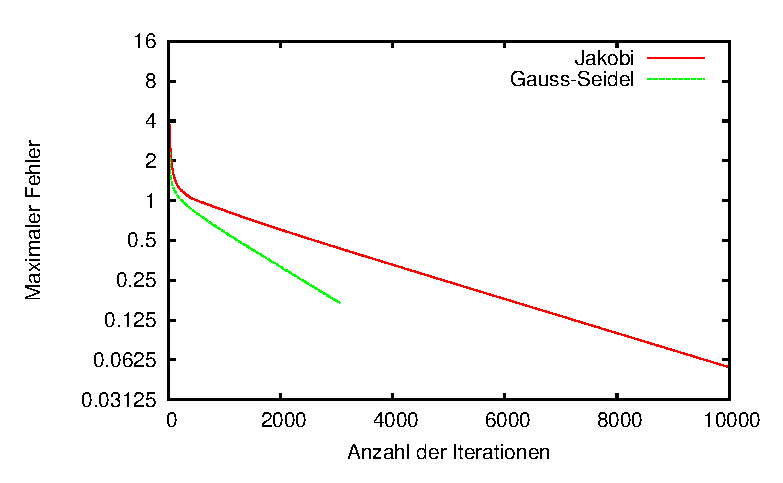
\includegraphics[width=\textwidth]{plots/fehlerpres}
\end{frame}

\section{Mehrgitter-Verfahren}
\subsection{Beschreibung}
\begin{frame}
    \frametitle{Mehrgitter"=Verfahren}
    Probleme bei den bisherigen Verfahren:
    \begin{itemize}
        \item Bei feinen Gittern dauern die einzelnen Iterationen zu lange
        \item Sowohl das Jakobi- als auch das Gauß-Seidel-Verfahren konvergieren nur langsam
    \end{itemize}
    Idee:
    \begin{itemize}
        \item Verbesserung des Startwertes durch Vorberechnungen auf gröberen Gittern
        \item Dadurch weniger Iterationen auf feinem Gitter nötig
    \end{itemize}
\end{frame}

\begin{frame}
    \frametitle{Mehrgitter"=Verfahren}
    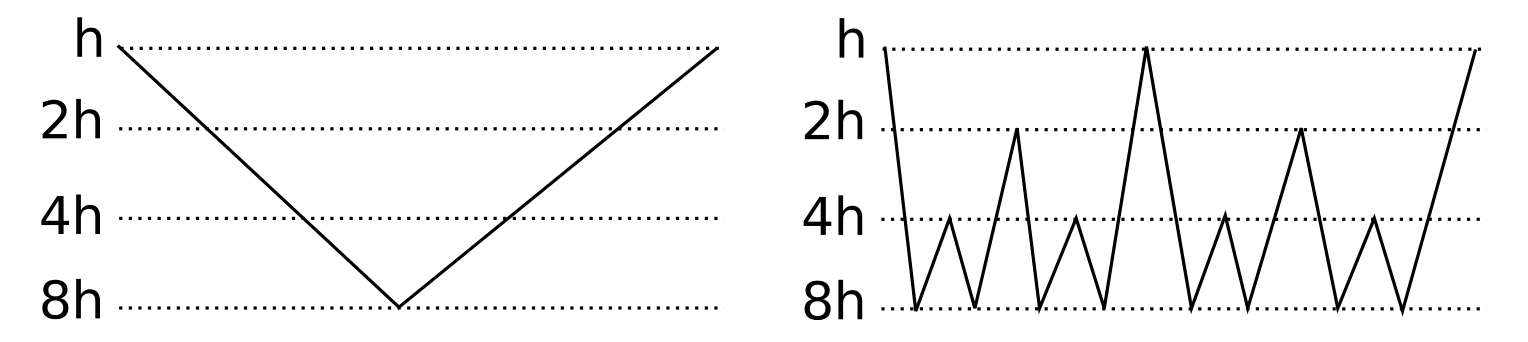
\includegraphics[width=\textwidth]{valgorithmus}

    Parameter:
    \begin{itemize}
        \item z1 / z2: Anzahl Iterationen bei der Glättung
        \item h-max: Wie grob wird das Gitter maximal
        \item alpha: Anzahl der Rekursionen
    \end{itemize}
\end{frame}

\begin{frame}
    \frametitle{Einfluss des Alpha"=Wertes}
    \framesubtitle{1000 Iterationen, $z = 4, hmax = 16 \cdot h$}
    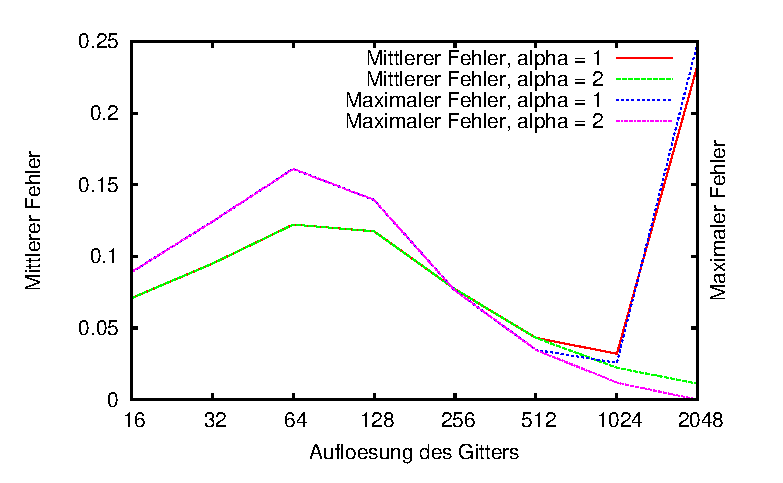
\includegraphics[width=\textwidth]{plots/fehlermehrgitter}
\end{frame}

\begin{frame}
    \frametitle{Restriktion und Interpolation}
    Grob nach fein: bilineare Interpolation
    
    Fein nach grob: Restriktion
    \begin{center}
        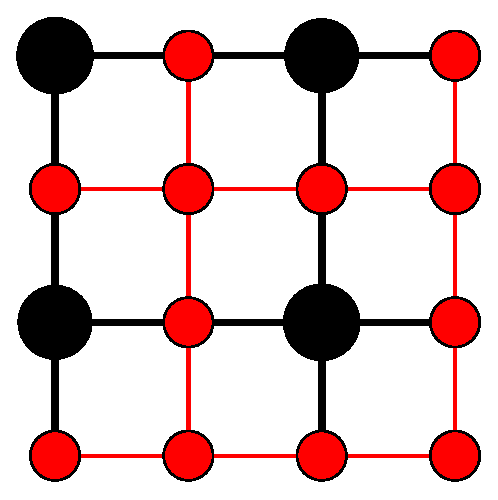
\includegraphics[width=0.4\textwidth]{interpolation}
    \end{center}
\end{frame}

\subsection{Grafisches Beispiel}
\begin{frame}
    \frametitle{Grafisches Beispiel}
    \framesubtitle{1000 Iterationen, $n=32, z=4, hmax=8 \cdot h, alpha=1$}
    \includegraphics<1>[trim=25 0 25 0, clip, width=\textwidth]{plots/000}
    \includegraphics<2>[trim=25 0 25 0, clip, width=\textwidth]{plots/001}
    \includegraphics<3>[trim=25 0 25 0, clip, width=\textwidth]{plots/002}
    \includegraphics<4>[trim=25 0 25 0, clip, width=\textwidth]{plots/003}
    \includegraphics<5>[trim=25 0 25 0, clip, width=\textwidth]{plots/004}
    \includegraphics<6>[trim=25 0 25 0, clip, width=\textwidth]{plots/005}
    \includegraphics<7>[trim=25 0 25 0, clip, width=\textwidth]{plots/006}
    \includegraphics<8>[trim=25 0 25 0, clip, width=\textwidth]{plots/007}
    \includegraphics<9>[trim=25 0 25 0, clip, width=\textwidth]{plots/008}
    \includegraphics<10>[trim=25 0 25 0, clip, width=\textwidth]{plots/009}
\end{frame}

\begin{frame}
    \frametitle{Interpolation}
    Besser wäre:
    \begin{center}
        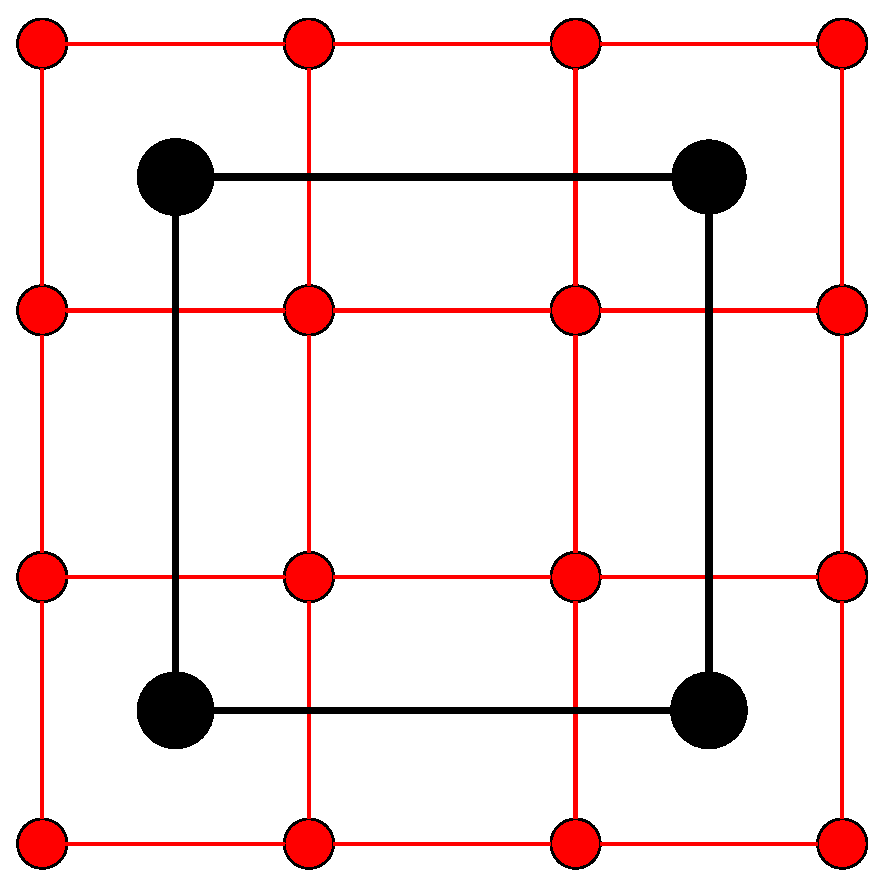
\includegraphics[width=0.5\textwidth]{interpolation2}
    \end{center}
\end{frame}

\subsection{Parallelisierung mit OpenMP}
\begin{frame}
    \frametitle{Parallelisierung Mehrgitter}
    Profiling: Aufrufe von Gauß-Seidel machen 95\% der Laufzeit aus
    \begin{itemize}
        \item Wiederverwendung der parallelen Gauß-Seidel Implementierung ist sinnvoll
        \item Interpolation und Restriktion haben keine Datenabhängigkeiten: trivial parallelisierbar
        \item Bei $alpha > 1$: Zwischen den rekursiven Aufrufen gibt es Datenabhängigkeiten
        \item Barrieren auch zwischen Glättung und Interpolation bzw. Restriktion notwendig
    \end{itemize}
\end{frame}

\begin{frame}
    \frametitle{Parallelisierung Mehrgitter: Effizienz}
    \framesubtitle{1000 Iterationen, $alpha=1$}
    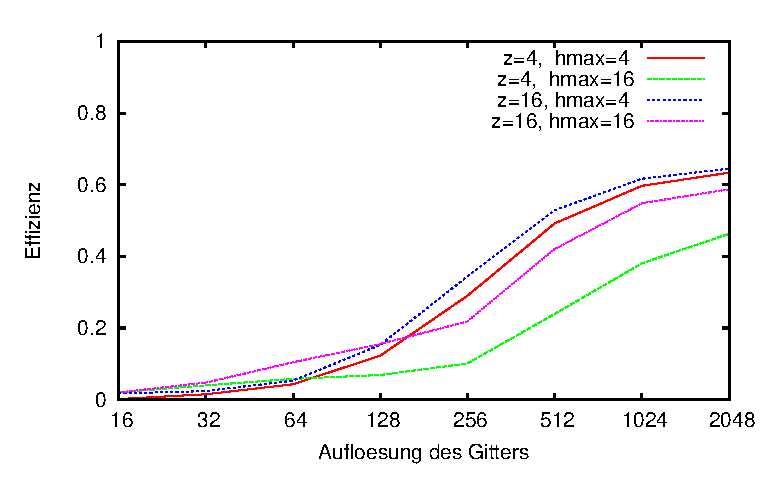
\includegraphics[width=\textwidth]{plots/effizienzmehrgitter}
\end{frame}

\section{Vergleich der Verfahren}
\subsection*{blubb}

\begin{frame}
    \frametitle{Effizienz}
    \framesubtitle{1000 Iterationen, $z=16, hmax=4, alpha=1$}
    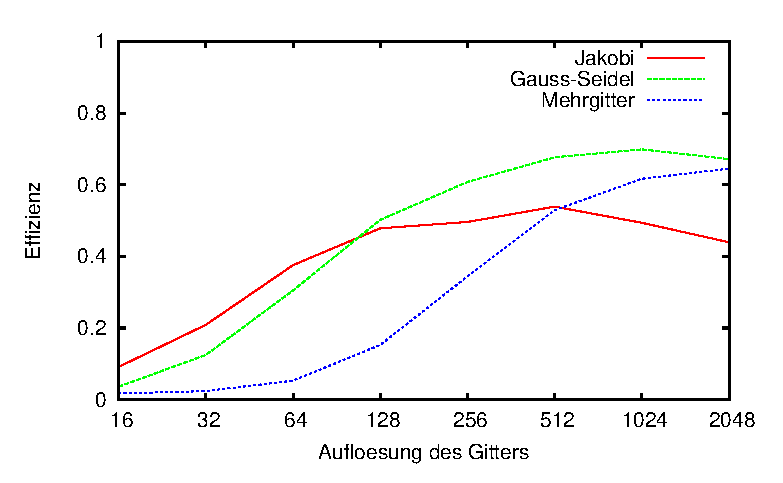
\includegraphics[width=\textwidth]{plots/effizienz}
\end{frame}

\begin{frame}
    \frametitle{Laufzeit sequentiell}
    \framesubtitle{1000 Iterationen, $z=16, hmax=4, alpha=1$}
    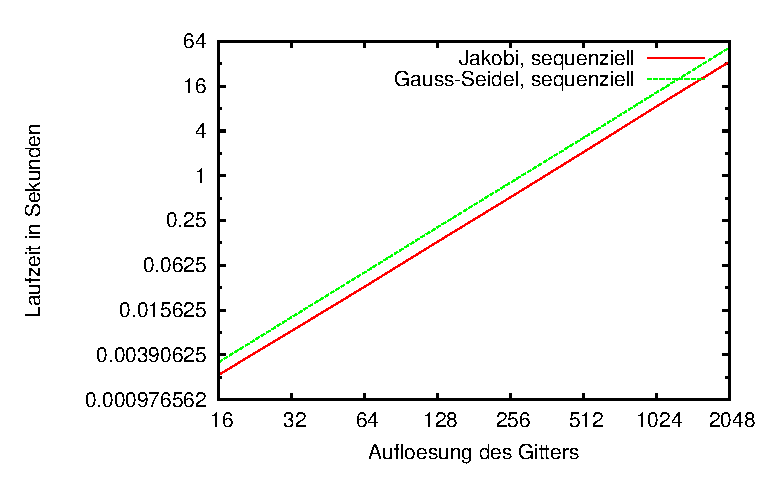
\includegraphics[width=\textwidth]{plots/laufzeitensequenziell}
\end{frame}

\begin{frame}
    \frametitle{Laufzeit parallel}
    \framesubtitle{1000 Iterationen, $z=16, hmax=4, alpha=1$}
    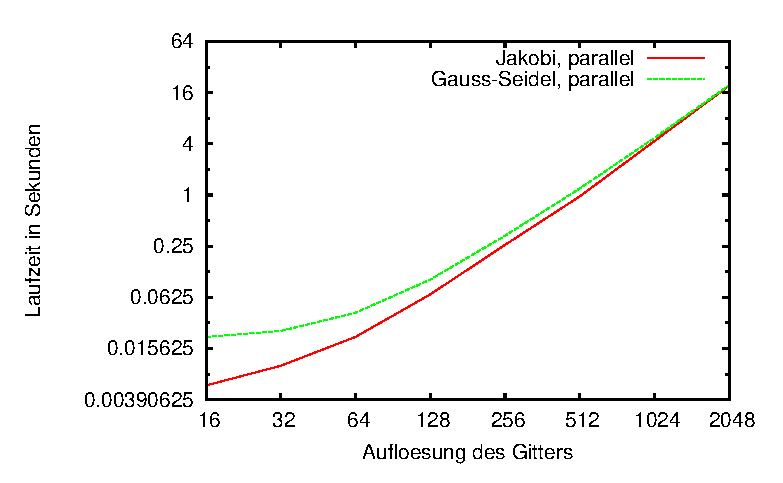
\includegraphics[width=\textwidth]{plots/laufzeitenparallel}
\end{frame}

\begin{frame}
    \frametitle{Mittlerer Fehler}
    \framesubtitle{1000 Iterationen, $z=16, hmax=4, alpha=1$}
    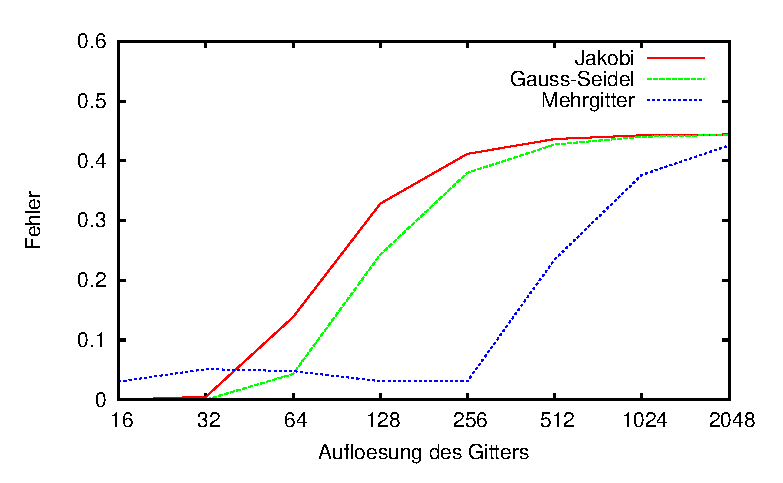
\includegraphics[width=\textwidth]{plots/fehlermittel}
\end{frame}

\end{document}
